\documentclass{article}
\usepackage[utf8]{inputenc}
\usepackage[T1]{fontenc}
\usepackage[a4paper,top=3.5cm,bottom=3.5cm,left=2.5cm,right=2.5cm,marginparwidth=1.75cm]{geometry}

\usepackage{amssymb}
\usepackage{amsmath}

\usepackage{graphicx}
\usepackage{svg}
\usepackage[french]{babel} 
\usepackage{multicol}
\usepackage{float}
\usepackage{fancyhdr}
\usepackage{booktabs}
\usepackage{hyperref}
\usepackage{cleveref}
\usepackage{subcaption}
\usepackage[labelfont=bf]{caption}

 
\pagestyle{fancy} 

\lhead{MINES ParisTech}
\chead{S3 Research internship}
\rhead{2018-2019}
\begin{document}
\begin{center}
    \begin{Large}\textbf{Gesture recognition using convolutional neural networks on skeletal data}\end{Large}

    \vspace{1cm}
    \begin{large}\underline{A.Thomas$^a$}, G.Devineau$^b$\end{large}

    \vspace{0.5cm}
    a. MINES ParisTech, alexandre.thomas@mines-paristech.fr\\
    a. MINES ParisTech CAOR, guillaume.devineau@mines-paristech.fr\\
    \vspace{1cm}
\end{center}

\noindent\textbf{Key words :} hand gesture recognition; convolutional networks; skeletal data; time sequences;
\\
\\
\textbf{Abstract : }
In this paper, we study different options to improve the performance of a deep learning model for 3D hand gesture recognition.
\par
We use a convolutional network to process the temporal sequences of skeletal joints positions, without using depth images. We compare a classical convolution network architecture with Temporal Convolution Network (TCN) architecture. We compare different activation functions.
We also study the impact of hyperparameters such as the batch size, the learning rate, the dropout, as well as the impact of changing the size and the depth of the network, or processing the channels separately.
\par
Experimental results on the DHG dataset from the SHREC17 Shape Retrieval Contest show that it is possible to achieve high accuracy with a relatively small and shallow convolution network (91.5\% in the 14 gesture classes case, 84.0\% in the 28 gesture classes case).


\section{Introduction}
\subsection{What kind of gesture recognition ?}
Gesture recognition is a way for humans to interact with machines without physical contact or voice command. Be it for device controlling without a remote (e.g. during driving or a medical operation) or for intelligent systems to understand humans intentions (e.g. pedestrians for autonomous driving \cite{intro-autonomous-driving} or for robot-human collaboration in a factory \cite{coupete:hal-01306482}), reliable and efficient algorithms for gesture recognition have an utility.
\par
There are multiple ways to do gesture recognition. One can simply use 2D data from a standard camera and extract features from the image. One can also use 3D-model based algorithms, which require more resources but have more potential. 3D data can be acquired with sensors (e.g. wired gloves track the motion of the hand, its position and the bending of the fingers), with depth-aware cameras or with stereo cameras.
\par
In order to deal with less parameters while keeping the essential information, skeletal representations of the body or the hand can be computed from 3D models. Even real-time pose estimation to detect keypoints of a body from images is possible (using special cameras such as Kinect \cite{real-time-human-pose-recognition-in-parts-from-a-single-depth-image}, or even with regular cameras \cite{simon2017hand-openpose}). For these reasons, our work is focused on gesture recognition using only 3D skeletal data sequences.
\par

\subsection{Existing approaches, ours}
Multiple approaches currently exist. For example, non-deep-learning methods with hand crafted features \cite{dhg-non-deep-approach}. However we choose to focus on deep learning methods, as the field has evolved a lot recently and shows promising results on various tasks, including gesture recognition with skeletal data \cite{Maghoumi-deep-gru}.
\par
Recurrent Neural Networks (RNNs) are usually the preferred approach to temporal sequences processing (as suggested by the title of the sequence modeling chapter in the reference textbook on deep learning : "Sequence Modeling : Recurrent and Recursive Nets" \cite{Goodfellow-et-al-2016}). However, other architectures such as Convolutional Neural Networks (CNNs) have also been successfully used for gesture recognition \cite{Devineau} or sequence modeling \cite{Bai2018-tcn}. As CNNs have potential advantages over RNNs, such as being more easily optimized in parallel or less sensitive to the first examples seen, we choose to explore this method and focus on convolutional networks.
\par
As a starting point, we use the model proposed by Devineau et al \cite{Devineau}, for gesture recognition on the DHG skeletal dataset \cite{dhg-non-deep-approach}. This network had state of the art results at the time (although now outperformed, cf \ref{section:results}), but had a relatively high total parameters count.
\par
Our aim is to improve the model architecture by improving its accuracy or reducing its total parameters count while keeping high accuracy. We explore and compare multiple options :
\begin{itemize}
    \item adding a preprocessing module (using a linear layer) on the temporal sequences before applying the convolutions, hoping to extract some meaning out of the sequences
    \item tweaking the architecture of the network (number of layers, number of separate channels, size of the layers, size of the fully-connected layers at the end, convolutions type)
    \item comparing different activation functions
\end{itemize}
We also explore a model based on Temporal Convolution Networks.


\section{Work}
In order to try new approaches, we end up with several possibilities at each layer, be it for the type of module used or the hyperparameters we choose. Let's detail, layer by layer, our options.

\subsection{Network architecture}
\subsubsection{Input data}
When working with 3D skeletal data, we are working with the spatial coordinates of $m$ skeletal joints $(j_i)_{i\in[1,m]}$. For each joint $j_i$, we have 3 temporal sequences of coordinates
$$(x^{(i)}(t), y^{(i)}(t), z^{(i)}(t))_{t\in \mathbb R}$$
As such, we define a 3D skeletal data sequence as a vector
$$s = (s_1 s_2 \dots s_n)^T$$
where $n=3m$ and where the variables $s_i$ are temporal sequences corresponding to the $x$, $y$ or $z$ coordinate of a joint.
In a skeletal representation of a 3D subject, the joints $j_i$ represent physical points of the subject body, such as articulations. Figure \ref{fig:hand-skeleton} gives an illustration of a 3D skeleton of the hand.
\begin{figure}
    \centering
    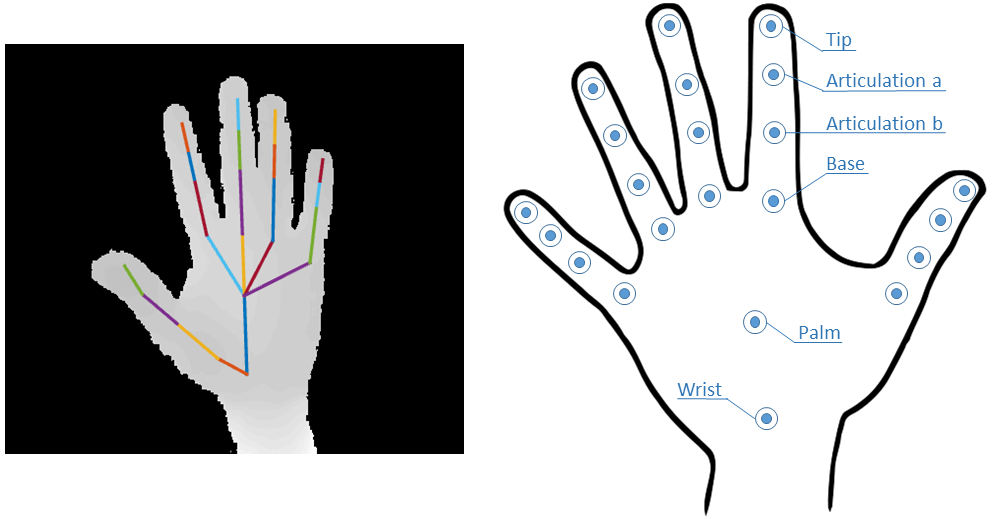
\includegraphics[width=0.5 \linewidth]{img/skeleton.png}
    \caption{\textit{The full skeleton returned by an Intel Real Sense Depth camera}}
    \label{fig:hand-skeleton}
\end{figure}
\par
Our experiments were done on the Dynamical Hand Gesture 14/28 (DHG) dataset \cite{dhg-non-deep-approach}. The dataset consists of 2800 labeled sequences, each corresponding to a hand gesture. The SHREC17 Challenge \cite{desmedt:shrec} introduced an evaluation protocol by separating the 2800 sequences dataset into a train set (70\%) and a test set (30\%). A total of 14 gestures are possible (\textit{Grab (G), Tap (T), Expand (E), Pinch (P), Rotation clockwise (RC), Rotation counter-clockwise (RCC), Swipe right (SR), Swipe left (SL), Swipe up (SU), Swipe down (SD), Swipe X (SX), Swipe + (S+), Swipe V (SV), Shake (Sh)}) and each gesture can be performed either using one finger or the whole hand. This makes a total of 14 or 28 label classes, depending on whether or not we consider the the 2 types of gestures as different label classes.
The hand skeleton contains $m=22$ joints, so each gesture consists of $n=66$ temporal sequences.
\par
The dataset sequences have different lengths, ranging mostly between 20 and 120 time steps (at 95\%). As our model requires fixed-sized inputs, we choose to resize all the sequences to a fixed length $L$. Different values of $L$ have been tried, in practice we chose $L=100$, which gave good results.
%TODO: check different values of L ?
In the end, our input data consists, for each test/train example, of $n$ data sequences $(s_1, s_2, \dots s_n)$ with
$$s_i = (s_i(t_0), s_i(t_1), \dots s_i(t_{L-1})), \forall i \in [1, n]$$
Figure \ref{fig:temporal-sequences} gives an example of such sequences.

\begin{figure}
    \centering
    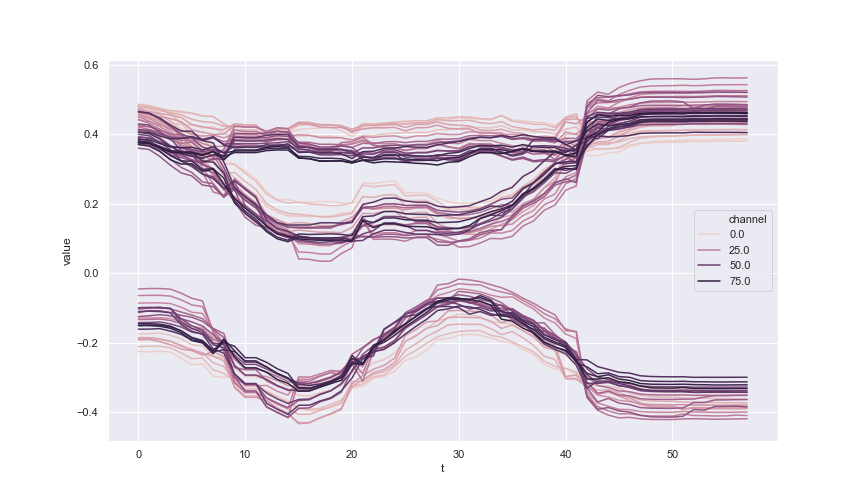
\includegraphics[width=0.7 \linewidth]{img/time_sequence_swipeX.png}
    \caption{\textit{Evolution of the data sequences $s_i$ for a Swipe X gesture, before resizing}}
    \label{fig:temporal-sequences}
\end{figure}

\subsubsection{Preprocessing module} \label{section:preprocessing-module}
The preprocessing module aimed at facilitating the work of the convolutional layers (described in \ref{section:convolutional-module}), maybe by extracting some meaning out of the input data.
The raw data distribution already had coherent, nearly normalized values (the data values range mostly from -0,6 to +0,8, with a mean of 0,18), so we did not feel the need to add a normalization layer during preprocessing.
\par
Let $x^{(i)}$ be a sequence example (i.e. an input tensor of shape $(L=100, C=66)$ for the DHG dataset), and $h_p$ the output of the preprocessing module. We tried the following options :

\paragraph{A linear module applying spatial combinations}
The idea here is to obtain linear combinations of the sequences $(s_i(t_k))_{k \in [0,L-1]}$. We hope that these linear combinations (allowing not only absolute joints coordinates, but also relative distances between the joints for instance, that could have higher semantic value) can be more easily exploited by the next layers.
\par
This layer is simply a linear transformation
$$h_p = A x^{(i)} + b$$
and we can choose the number of output channels $C_{p,out}$, so that output of the preprocessing layer $h_p$ has $(L, C_{p,out})$ shape.
% \item \textbf{A graph convolution layer} (\emph{graph-conv}).
% From the beginning we represented our temporal sequences as a simple tensor with $n$ channels. However the different joints have physical links and the skeleton can also be seen as a graph with one node per joint (just like in figure \ref{fig:hand-skeleton}). In this representation we have $m$ nodes, each of the node $j$ being assigned 3 feature channels, for the $x_j$, $y_j$ and $z_j$ temporal sequences.
% TODO : faire un preprocessing de graph qui a du sens ?? ça c'est pour du semi-supervised learning, rien à voir

\paragraph{No preprocessing module}
The input sequences were directly processed by the convolutional module.

\subsubsection{Convolutional module} \label{section:convolutional-module}
The convolutional module does most of the work by extracting important features out of the sequences, before the final classification module. We explore here 2 options :
\paragraph{A regular 1D Convolutional network} based on the multi-channel convolutional neural network proposed by Devineau et al. \cite{Devineau}.
\par
The initial network (explained with more details in \cite{Devineau}) was based on multiple parallel and independant modules : for each channel $i \in [1,n]$, the sequence $s_i$ would be processed separately by a channel-specific module before being concatenated to the other channel-specific outputs and processed by the classification module. Each channel-specific module consisted of 3 parallel branches :
\begin{itemize}
    \item A high-resolution convolutional branch, consisting of several 1D convolutions with pooling, with a "high" kernel size ($k=7$ in the paper).
    \item A low-resolution convolutional branch, identical to the high resolution except for the kernel size ($k=3$ in the paper).
    \item A residual branch that is almost an identity function with some pooling. It has been found that residual branches can help optimizing deep networks and improving accuracy \cite{He_2016-residual}, and it seemed to have a small but favorable impact on our initial network \cite{Devineau}, especially in the 28-gestures case.
\end{itemize}
\par
In our regular convolutional module, we keep these ideas (high and low-resolution branches, residual branches) but we want to study a more flexible architecture.
\par
Our convolutional module is made of 2 parallel branches, each one working at a different resolution (kernel size $k=3$ for the small branch, $k=7$ for the high branch). Their outputs are finally concatenated into a single vector, for the classification module.
\par
Both branches are made of multiple convolutional blocks, one after the other. The architecture of a convolutional block is illustrated in figure \ref{fig:regular-conv-block-architecture}.
\begin{figure}
    \centering
    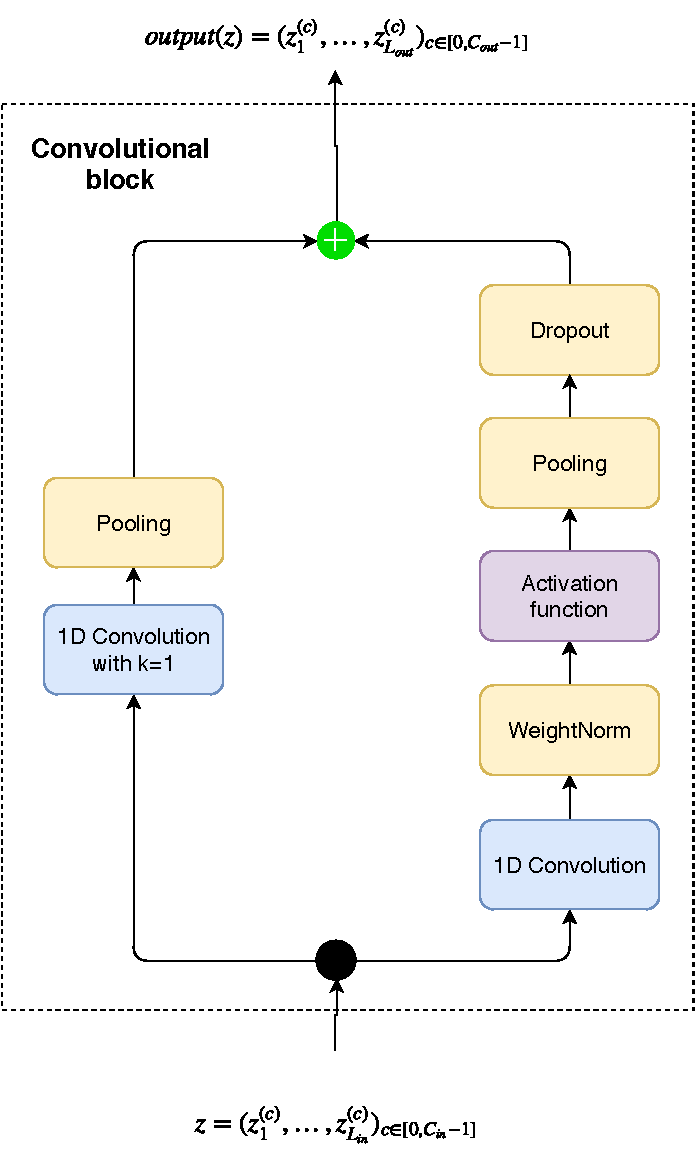
\includegraphics[scale=0.5]{img/residual_block.pdf}
    \caption{\textit{Architecture of a regular convolution block. Kernel size can be $k=3$ or $k=7$ depending on the branch, and the \emph{groups} parameter allows the 1D Conv block to process inputs independantly}}
    \label{fig:regular-conv-block-architecture}
\end{figure}

\begin{figure}
    \begin{subfigure}{.49\linewidth}
        \centering
        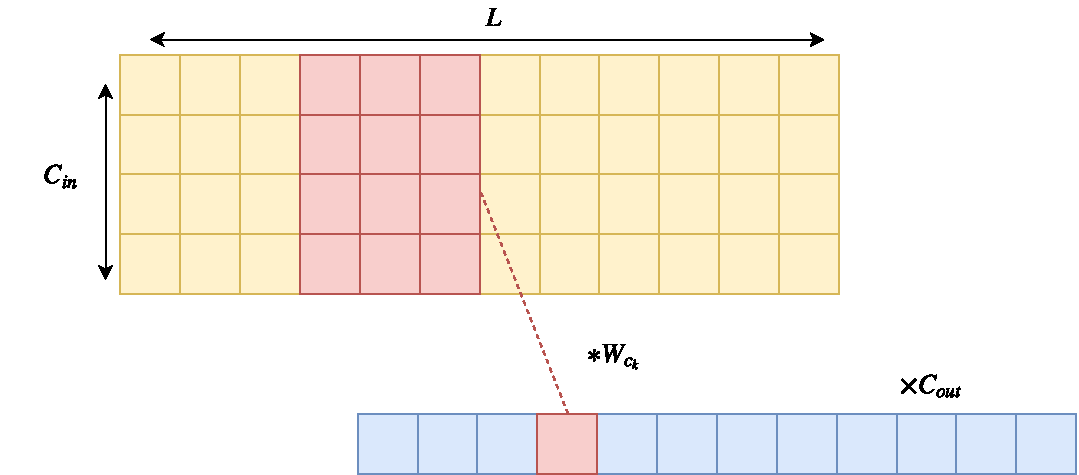
\includegraphics[width=.8\linewidth]{img/1D-conv.pdf}
        \caption{\textit{A regular 1D convolution layer}}
        \label{fig:regular-conv-layer}
    \end{subfigure}
    \begin{subfigure}{.49\linewidth}
        \centering
        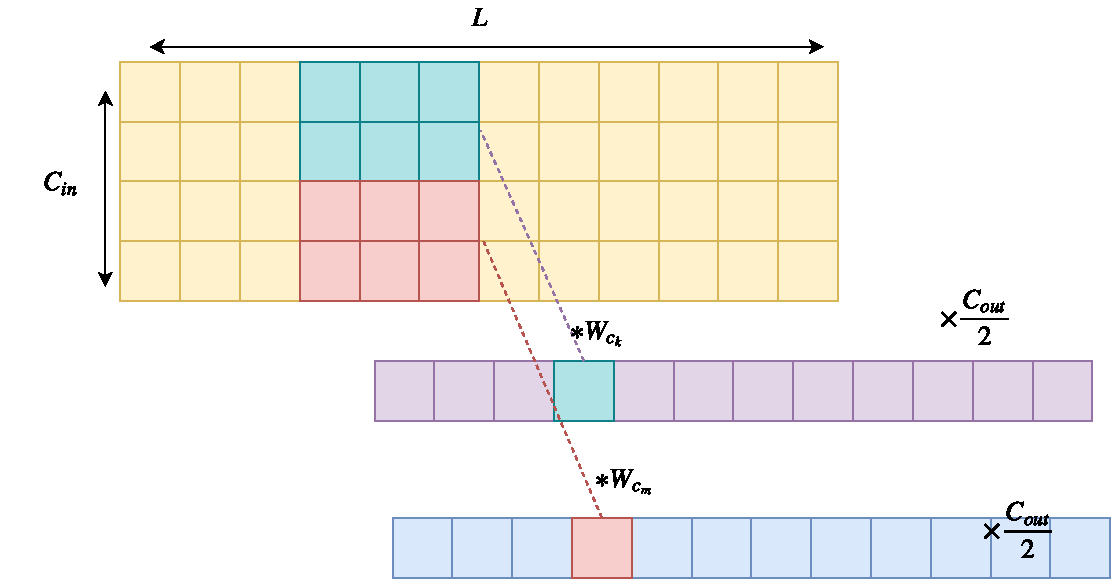
\includegraphics[width=.8\linewidth]{img/1D-conv-groups.pdf}
        \caption{\textit{A regular 1D convolution layer, with $groups=2$ (instead of 1, by default). Half of the inputs are convolved to produce half of the outputs, independantly}}
        \label{fig:regular-conv-layer-with-groups}
    \end{subfigure}
    \caption{\textit{Illustration of regular 1D convolutions}}
\end{figure}

Each block is made of :
\begin{enumerate}
    \item \emph{A classical 1D convolution transformation}
    \par
    Let $C_{in}$ be the number of input channels, $C_{out}$ the number of output channels, $(z^{(c)})_{c \in [0, C_{in}-1]}$ the input sequences. The outputs of a 1D convolution layer are calculated as :
    $$(output(z))^{(c_o)} = \sum_{c_i=0}^{C_{in}-1} W_{c_o}^{(c_i)} * z^{(c_i)} + b_{c_o}$$
    Where $c_o \in [0, C_{out}-1]$ is the index of the output sequence, $W_{c_o}$ the convolution filter of output channel $c_o$ and $b_{c_o}$ the bias.
    Figure \ref{fig:regular-conv-layer} illustrates this.
    \par
    Kernel size is $k=3$ or $k=7$ depending on the resolution, and zero-padding is applied on both ends of the input to obtain same-length sequences.
    For each convolutional block (which can be seen as a layer), the number of outputs $C_{out}$ can be chosen as a hyperparameter.
    \par
    The other major hyperparameter here is the \emph{groups} parameter, which controls the connection between inputs and outputs, and allows to treat channels independantly.
    For instance, having $groups=2$ is equivalent to having two 1D convolution layers side by side, each one seeing half of the inputs and producing half of the outputs. Having $groups=C_{in}$ is equivalent to having $C_{in}$ separate convolution layers, each one seeing only one input channel, just like our initial network architecture.
    Figure \ref{fig:regular-conv-layer-with-groups} illustrates this mechanism.
    \par
    Having independant convolution weights for each input channel allows the initial network to perform well, however it may require a high number of parameters. It is likely that some input channels share similar information and therefore we could possibly share convolution weights between the channels while keeping comparable accuracy. This would greatly reduce the total number of model parameters.
    \par
    Finally, we add a weight normalization layer to accelerate training \cite{salimans2016weight}, an activation function for non-linearity, a pooling layer and dropout regularization.
    
    \item \emph{A residual connection}
    \par
    As stated earlier, we add a residual connection to the output of the convolution as it tends to improve accuracy and facilitate the training of deep networks. However, after the convolution transformation, the shape of tensor $output(z)$ is usually modified, both regarding the number of channels (if we choose $C_{out} \neq C_{in}$) and the length of the sequence (because of pooling).
    \par
    In order to still be able to add $z$ and $output(z)$, we use a 1D convolution with kernel size $k=1$ to change the number of channels without transforming the sequences in the temporal space, and we use average pooling to change the length of the sequences accordingly.
    
\end{enumerate}

\paragraph{A Temporal Convolutional network (\emph{TCN})} \label{section:tcn} based on a slightly different architecture proposed by \cite{Bai2018-tcn} for sequence modeling tasks (given a sequence of elements, the goal is to predict the next element of the sequence).
\par
Both architectures (our classical 1D convolution and TCN) use convolutional layers to process the sequence and produce multiple output channels.
Our classical architecture detailed above takes a number of fixed size sequences as input and outputs several sequences that are usually shorter ($L_{out} < L_{in}$), the goal being to synthetize information for the classification layer. The full output sequences are then processed by the classification layer. The fixed-size input sequences can be either the full gestures (offline gesture recognition), or the last timesteps recorded up to time $T$ (online, real-time gesture recognition).
\par
The TCN architecture is made to work on online data. The inputs are still fixed size sequences and the network outputs multiple sequences $(y^{(c)})_{c \in [0, C_{out}-1]}$ of same size ($L_{out} = L_{in} = L$). However only the last timestep $(y^{(c)}(t=L))_{c \in [0, C_{out}-1]}$ is processed by the classification layer and used for training and/or evaluating.
The network uses dilated convolutions so that even a single output sequence element is represents widespread input data, and therefore keeps a long memory (more details in \cite{Bai2018-tcn}).
\par
The results looked promising on various sequence modeling tasks, achieving or surpassing recurrent networks. Although our goal is to classify temporal sequences and not predict the next element, the task still requires the network to gain an understanding of the input sequences and have a memory of the past time steps. Furthermore, even though we did not have the time to really explore real-time gesture classification, we initially wanted to and this kind of architecture seemed interesting.
%TODO : refaire les tests de performance du tcn, cette fois en ne prenant que le dernier timestep dans la séquence produite (cf https://github.com/locuslab/TCN/tree/master/TCN/poly_music)

\subsubsection{Classification module} \label{section:classification-module}
Finally, we use a multi layer perceptron (MLP) for classification. The outputs of low and high resolution convolution branches are concatenated, and flattened into a 1D tensor, of size $L_{out} \times C_{out} \times 2$. Figure \ref{fig:mlp-classification-module} illustrates the architecture. The choice of the number of hidden layers (one or more) and their size is left as an hyperparameter.

\begin{figure}
    \centering
    \includeinkscape[width=0.5\linewidth]{img/mlp}
    \caption{Schematic illustration of the MLP used for classification. There are $L_{out} \times C_{out} \times 2$ inputs and as many outputs as the number of classes (14 or 28 for the DHG dataset). There can be one or more hidden layer, each of size $n_{hidden}^{(i)}$.}
    \label{fig:mlp-classification-module}
\end{figure}

\subsection{Hyperparameters}
For the cost function, we choose the commonly used negative log likelihood loss. For the optimization algorithm, we use the Adam optimizer, a stochastic gradient descent algorithm with adaptative learning rate \cite{kingma2014adam} known to perform well in most situations \cite{Ruder2016-gradient-descent-algos-overview}. Weight initialization can help a lot to converge, so we use Xavier initialization \cite{xavier-init} instead of random initilization.
\par
In addition to the hyperparameters detailed in previous sections, that will define our model architecture, we also have to choose a few other classical hyperparameters in deep learning. Here they are, with the set of values we would like to try.

\begin{itemize}
    \item \emph{Number of epochs}
    \par
    In order to prevent overfitting on the training set, it is important to stop the training once the validation score stops improving. Therefore, we use early stopping to automatically stop training if validation loss did not improve during the last 50 steps by at least 0,01\%.
    \item \emph{Batch size} \label{section:batch-size}
    \par
    32, 64, \dots, 512 are frequently used batch sizes. Higher batch sizes are quicker to process during training on GPU, however it has been found that it can lead to poorer generalization \cite{keskar2016largebatch}. In stochastic gradient descent algorithms, the gradient is averaged over a batch and larger batches seem to converge more sharply to local optimas, in comparison to smaller batches which are noisier. Therefore, we try a range of values : $batch\_size \in [8, 16, 32, 64, 128, 256, 512]$
    \item \emph{Learning rate}
    \par
    By default it is suggested to use 0,001 with the Adam optimizer, but we found that decreasing the initial learning rate lead to more stable training. Therefore, we try a few different values.
    \item \emph{Activation function} \label{section:act-fct}
    \par
    The ReLU function (Rectified Linear Unit) $ReLU(x) = max(0,x)$ is the standard activation function. However we try two other promising options :
    \begin{enumerate}
        \item The Parametric Rectified Linear Unit (PReLU), a variant of the ReLU function : $PReLU(x) = max(0,x) + \lambda min(0,x)$, where $\lambda$ is a parameter learned during training. This function, introduced by \cite{He_2015-prelu}, aims to improve ReLU by avoiding zero gradients, while adapting the negative slope for every layer.
        \item The Swish function : $Swish(x) = x \cdot sigmoid(\beta x)$, where $\beta$ is a constant or trainable parameter. This function, introduced by \cite{ramach2017-swish}, seemed to work better than ReLU on a number of datasets. In order to avoid adding a hyperparameter, we make $\beta$ a trainable parameter, just like the $\lambda$ parameter of PReLU.
    \end{enumerate}
    \item \emph{Dropout}
    \par
    We use dropout as a regularizer, and we try different values for the drop rate $p \in [0,1]$.
\end{itemize}


\section{Results}

\subsection{Implementation}
The network was implemented with PyTorch\footnote{Code can be found at \url{https://github.com/alexandrethm/S3R}}, and we used GPU acceleration when possible to speed up training : with a high enough batch size ($\geq 64$), we were able to train most models in a few minutes with a few hundreds to a thousand epochs.
\par
The DHG dataset is already splitted in a train and a test dataset. However, as we want to evaluate multiple different architectures and hyperparameters, we must avoid using the test dataset to select these hyperparameters, otherwise we might overfit. 
Therefore, we use stratified 3-fold cross-validation to evaluate and compare our different model architectures. Most of the following scores are mean accuracy of the model across the 3 validation sets.
The test dataset is only used for final evaluation, once the architecture and the hyperparameters are chosen.
\par
Many experiments (using both grid searches and randomized searches) were conducted to find good-performing architectures. We found that the following values worked well on the DHG dataset, so we take them as default in the next sections, and only change one or two hyperparameters at a time :
\begin{equation}
    \begin{aligned}
        & batch\_size=128 ; learning\_rate=10^{-4} ; dropout=0,4; \\
        & activation\_function=PReLU ; preprocess=None ; conv\_type=regular            
    \end{aligned}
\end{equation}
with 1 convolution layer $(C_{out}=22, groups=1)$ and two hidden fully-connected layers of size $(N_{out, 1}=1024, N_{out, 2}=128)$.


\subsection{Convolutional module}
\paragraph{How to size the network ?} \label{section:conv-size}
We want to find out how deep our network should be (number of convolution layers), and how much channels should there be per layer.
Randomized searches gave us some good performing architectures, but in order to have more insight on the role of these parameters, we try a more extensive grid search with $n \in \{1, 2, 3, 4\}$ convolution layers and $C_{out} \in \{11, 22, 44, 66, 96\}$ output channels per layer.
Results are presented in figure \ref{fig:conv-size}.
\begin{figure}
    \centering
    \begin{subfigure}{0.45\linewidth}
        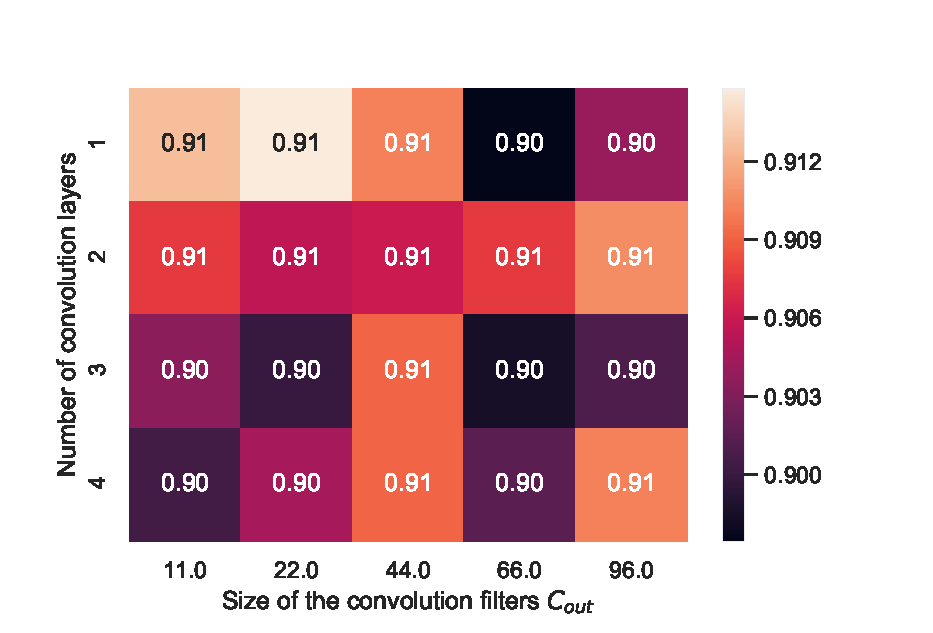
\includegraphics[width=\linewidth]{img/heatmap-conv-layers-nb-size.eps}
        \caption{Mean accuracy of different convolution architectures on the validation set (using 3-fold cross-validation)}
        \label{fig:heatmap-conv-layers-nb-size}            
    \end{subfigure}
    \begin{subfigure}{0.45\linewidth}
        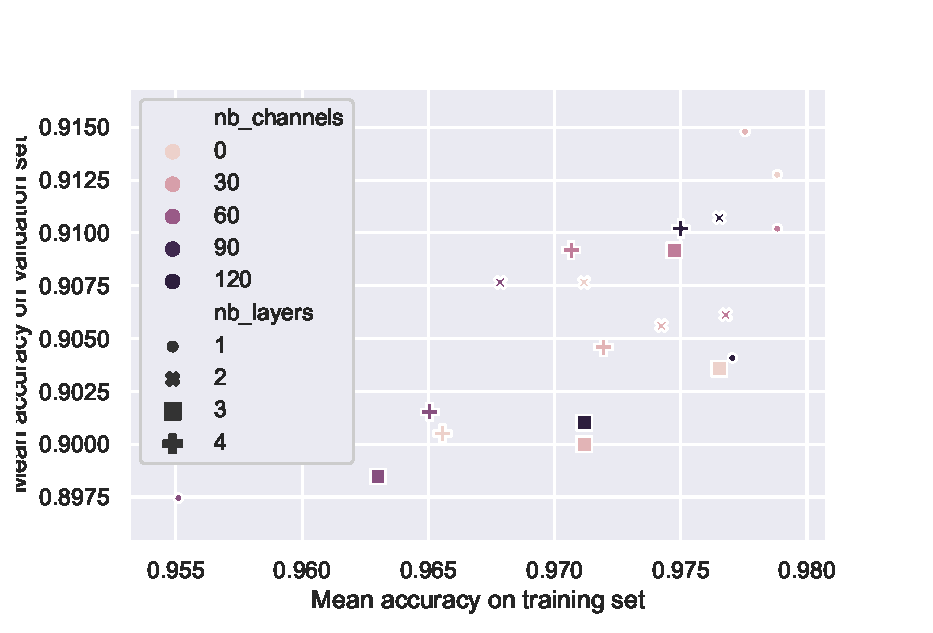
\includegraphics[width=\linewidth]{img/scatter-conv-layers-nb-size.eps}
        \caption{Mean accuracy on the validation set (y-axis) and the training set (x-axis). Models in the bottom right part of the graph are more likely to overfit on the training set.}
        \label{fig:scatter-conv-layers-nb-size}            
    \end{subfigure}
    \caption{Influence of the number and the size of convolution layers on accuracy.}
    \label{fig:conv-size}
\end{figure}
\par
It seems that small and shallow architectures perform better, meaning :
\begin{itemize}
    \item A deep network is not necessary. When the convolutions are small ($C_{out} \in \{11, 22\}$), adding more layers generally decreases validation accuracy. When $C_{out} \geq 44$, no trend seems visible.
    \item A large network (with many convolution channels and parameters) is not necessary. Good performance is achieved with various $C_{out}$, with $C_{out}=22$ having the best overall score.
\end{itemize}
Figure \ref{fig:scatter-conv-layers-nb-size} shows that small and shallow architectures ($C_{out} \in \{11, 22\}$ and $n=1$) have better scores on both validation and training set. This suggests that they generalize better (higher validation accuracy) but also converge more easily (higher training accuracy).
It should be noted however that we are working on a relatively small dataset, and that deeper architectures may be necessary for datasets with more examples and classes.

\paragraph{The \emph{groups} parameter}
The initial network \cite{Devineau} was using 66 parallel convolution networks, each one having 3 layers of size $C_{out}=(8,8,4)$ and having 1 input sequence. This is the same as having the following 3 layers 
$$[(C_{out}=66\times 8, groups=66), (C_{out}=66\times 8, groups=66), (C_{out}=66\times 4, groups=66)]$$
working on all 66 input sequences.
Section \ref{section:conv-size} suggests that having this many channels and this many layers is not necessary, at least on the DHG dataset.
We still want to see how this $groups$ parameter affects our model, and if some sequences separately improves the performance.
\par
Figure \ref{fig:groups-parameter} presents some results. 
The role of processing input sequences separately rather does not seem obvious here, at least for relatively small architectures such as ours. Nonetheless, it does not seem to improve accuracy, so we choose to stick with classical convolution layers ($groups=1$).
\begin{figure}
    \centering
    \begin{subfigure}{0.45\linewidth}
        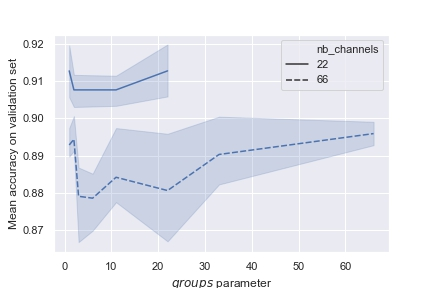
\includegraphics[width=\linewidth]{img/groups-param-nb-channels.jpg}
        \caption{Here we have 1-layer architectures, with either 22 or 66 output channels}
    \end{subfigure}
    \begin{subfigure}{0.45\linewidth}
        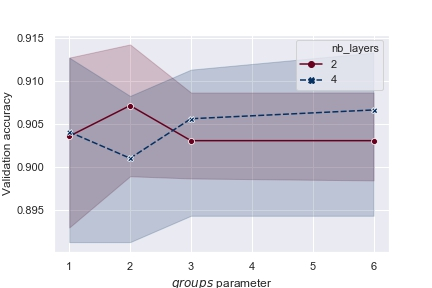
\includegraphics[width=\linewidth]{img/groups-param-nb-layers.jpg}
        \caption{Here we have 2 or 4-layer architectures, with 96 output channels for each layer. The values $groups$ can take are limited because it must divide 66 and 96}
    \end{subfigure}
    \caption{Influence of the $groups$ parameter on accuracy. Each one of the $C_{out}$ convolutions sees only $\frac{66}{groups}$ input sequences. $groups=1$ is a classical convolution layer, $groups=66$ means that input sequences are processed independantly. \\ The average score on the 3 splits of the cross-validation is taken, and the blue bars represent the 95\% confidence interval.}
    \label{fig:groups-parameter}
\end{figure}
\par

\paragraph{What about TCNs ?}
Here, the architecture is slightly different from our classical convolution network, as described in \ref{section:tcn}. Furthermore, we do not have 2 separate branches working with different filter sizes $k$, but only one branch.
We explore 3 essential hyper-parameters :
\begin{itemize}
    \item The depth $d$ of the network, i.e. the number of successive convolution layers
    \item The number of convolution channels per layer $C_{out}$
    \item The filter size $k$ of the convolutions \footnote{This is new compared to the previous paragraph with regular CNNs, where our model had 2 branches with fixed filter size $k=3$ and $k=7$}
\end{itemize}
Experimental results (figure \ref{fig:tcn}) suggest that :
\begin{itemize}
    \item TCNs require more depth than our classical CNN to be accurate (at least 5 layers). Cf figure \ref{fig:tcn_nb_layers}.
    \item Having large networks with a high $C_{out} (\geq 200)$ enables good performance (cf figure \ref{fig:tcn_nb_channels}). Other experiments with lower $C_{out}$ (not shown here) did not perform that well.
    \item A minimum kernel size is required to perform well, presumably for the model to have a long enough memory. We see that, with $d=5$ layers, kernel size $k=2$ (giving a receptive field of $k^d=2^5=32$ timesteps to the network) is not sufficient, whereas $k=3$ (giving a receptive field of $k^d=3^5=243$) is enough (cf figure \ref{fig:tcn_kernel_size}).
\end{itemize}
\par
Note that, in the TCN case, the classification module's input is only the last timestep output $(y^{(c)}(t=L))_{c \in [0, C_{out}-1]}$, of size $C_{out}$ (number of channels output of the last convolution layer), whereas the size is $(C_{out}, L_{out})$ for our regular CNN model. Even though we choose a larger $C_{out}$ than in the regular CNN architecture, the output of the convolution module is much smaller. Therefore we use a MLP with only one hidden layer (of size 128) for classification.
\par
Another remark we can make is that, although results are comparable to the regular CNN model, the TCN model has considerably more parameters and is much slower to train (~20 times slower than a small and shallow CNN architecture), as most of the output is not used for classification.
\begin{figure}
    \centering
    \begin{subfigure}{0.45\linewidth}
        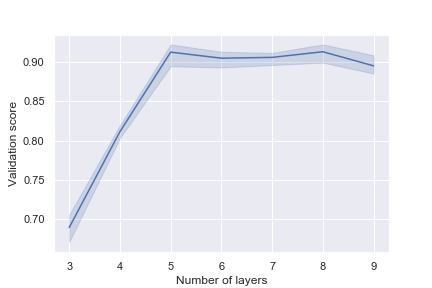
\includegraphics[width=\linewidth]{img/tcn_nb_layers.png}
        \caption{Here the number of channels per convolution layer is set to $C_{out}=300$ and we change the number of layers}
        \label{fig:tcn_nb_layers}            
    \end{subfigure}
    \begin{subfigure}{0.45\linewidth}
        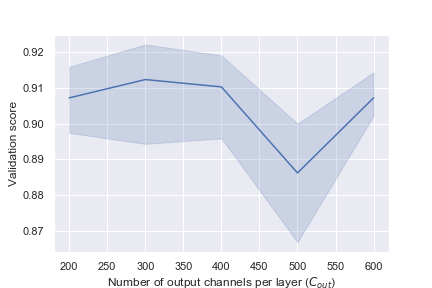
\includegraphics[width=\linewidth]{img/tcn_nb_channels.png}
        \caption{Here the number of layers is set to $d=5$ and we change the number of output channels per layer}
        \label{fig:tcn_nb_channels}            
    \end{subfigure}
    \begin{subfigure}{0.45\linewidth}
        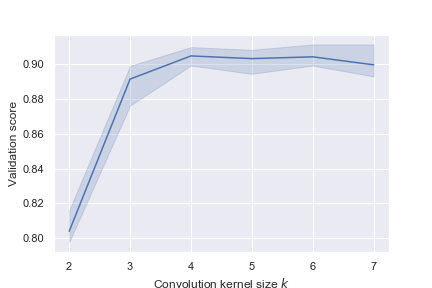
\includegraphics[width=\linewidth]{img/tcn_kernel_size.png}
        \caption{Here we have 5 layers with $C_{out}=300$ output channels, and we change the kernel size (previously set to 3)}
        \label{fig:tcn_kernel_size}            
    \end{subfigure}
    \caption{Experiments on TCNs architectures}
    \label{fig:tcn}
\end{figure}


\subsection{Preprocessing module}
Here we try to add linear spatial combinations of the 66 input sequences before the convolution layers (as detailed in \ref{section:preprocessing-module}). We keep the reference architecture (1 convolution layer with $C_{out}=22$ and $groups=1$) and we try various sizes of the linear layer, with 22 to 132 channels out.
\par
The results (figure \ref{fig:preprocessing}) seem to indicate that adding this layer has no particular effect on the accuracy.
\begin{figure}
    \centering
    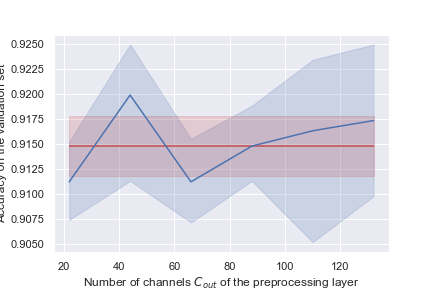
\includegraphics[width=0.6\linewidth]{img/preprocessing.png}
    \caption{Accuracy obtained with various sizes of the linear preprocessing module (blue curve). The red line is the reference architecture, without a preprocessing module.}
    \label{fig:preprocessing}
\end{figure}

\subsection{Classification module}
After the convolution network, we use a MLP (described in \ref{section:classification-module}) with 1 or 2 fully connected hidden layers, of various sizes (the number of hidden units in a layer). Figure \ref{fig:fc_layers} shows the results of the experiments.
\par
It seems that :
\begin{itemize}
    \item having 2 layers gives slightly better results
    \item the 2 layers should not have too many parameters : the biggest architectures ($fc\_layer\_0=2048$ and $fc\_layer\_1=512$ for instance) perform slightly worse than the others.
\end{itemize}
Apart from that, there does not seem to be a clear optimum : our choice of $fc\_layer\_0=1024$ and $fc\_layer\_1=128$ seems acceptable.
\begin{figure}
    \centering
    \begin{subfigure}{0.6\linewidth}
        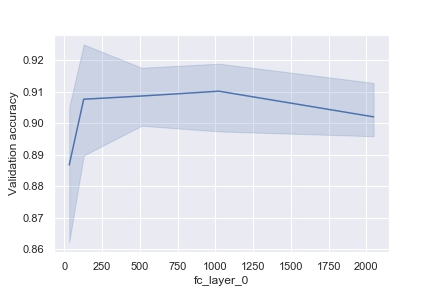
\includegraphics[width=\linewidth]{img/1_fc_layers.jpg}
        \caption{Here we have only 1 hidden layer, and we change its size $fc\_layer\_0 \in \{32, 128, 512, 1024, 2048\}$.}
    \end{subfigure}
    \begin{subfigure}{\linewidth}
        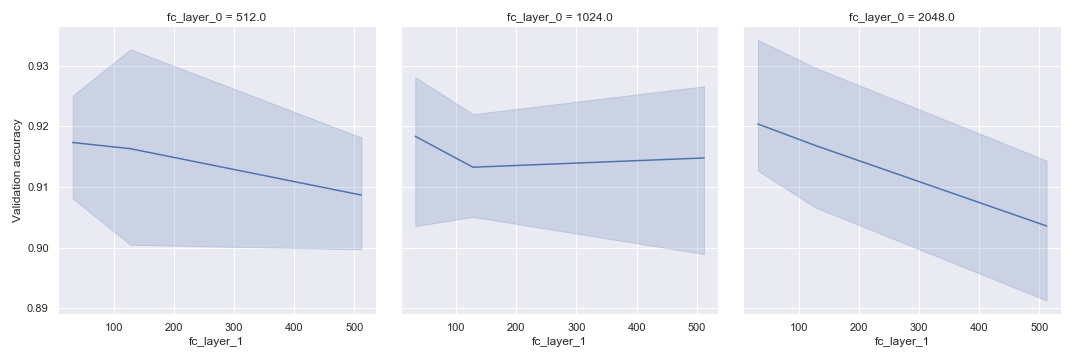
\includegraphics[width=\linewidth]{img/2_fc_layers.jpg}
        \caption{Here we have 2 hidden layers and we try different combinations of their sizes $fc\_layer\_0$ and $fc\_layer\_1$.}
    \end{subfigure}
    \caption{Experiments on the size and the depth of the MLP we use for classification}
    \label{fig:fc_layers}
\end{figure}

\subsection{Other hyperparameters}
\paragraph{Batch size}
% 64 seems optimal
Here we try $batch\_size \in [8, 16, 32, 64, 128, 256, 512]$, and figure \ref{fig:batch-size} shows the results. Although a bit chaotic, we find that :
\begin{itemize}
    \item Usual batch sizes (64 to 512) work generally fine
    \item Accuracy indeed starts decreasing when batch sizes get too big (after 1024)
\end{itemize}
\begin{figure}
    \centering
    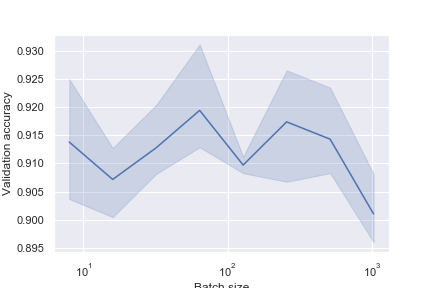
\includegraphics[width=0.6\linewidth]{img/batch_size.png}
    \caption{Experiments on the batch size}
    \label{fig:batch-size}
\end{figure}

\paragraph{Learning rate}
% 5e-5 seems optimal
Results are shown in figure \ref{fig:learning-rate}. The optimal value seems to differ a bit from the default value proposed for Adam optimizer \cite{kingma2014adam}, being around $lr=5\times10^{-5}$ in our case. Models with learning rates too low have difficulty converging, while models with learning rates too high have difficulty finding the optimum (we found that accuracy fell sharply to $0.6$ when $lr\geq5\times10^{-3}$ — not shown in the figure).
\begin{figure}
    \centering
    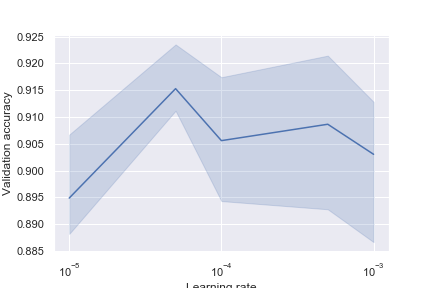
\includegraphics[width=0.6\linewidth]{img/learning_rate.png}
    \caption{Experiments on the learning rate}
    \label{fig:learning-rate}
\end{figure}

\paragraph{Activation function}
Trying the different activation functions detailed in \ref{section:act-fct}, we find that the \emph{PReLU} \cite{He_2015-prelu} and the \emph{Swish} \cite{ramach2017-swish} activation functions perform better than the classical \emph{ReLU} function (results in figure \ref{fig:act-fct}).
\begin{figure}
    \centering
    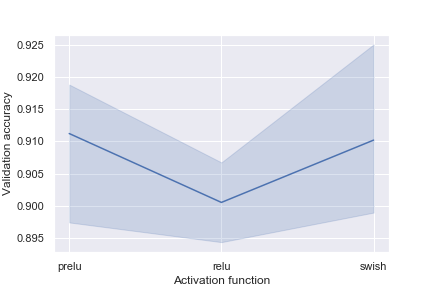
\includegraphics[width=0.6\linewidth]{img/act_fct.png}
    \caption{Comparison of different activation functions}
    \label{fig:act-fct}
\end{figure}

\paragraph{Dropout}
% 0.5 seems optimal
Here we try different values of dropout, from 0 to 0.8 (figure \ref{fig:dropout}), and we find that dropout is an effective regularization technique and improves our model's accuracy (up to +2.5\%).
\begin{figure}
    \centering
    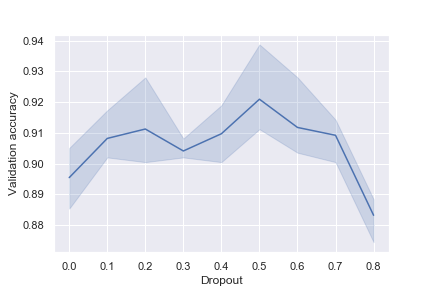
\includegraphics[width=0.6\linewidth]{img/dropout.png}
    \caption{Experiments on the dropout}
    \label{fig:dropout}
\end{figure}

\subsection{Results on the DHG dataset} \label{section:results}
In the end, after adjusting our initial architecture according to the above sections, we find — in the 14-gestures case and with the regular CNN architecture — a mean accuracy of
$$valid\_acc = 0.918 \pm 0.006$$
on our validation datasets, when doing 3-fold cross-validation (95\% confidence interval).
\par
Now that the architecture is chosen, we can test our models against the test dataset (both the regular CNN architecture and the TCN architecture).
Results are shown in the table \ref{tab:results}.
We can see that our models are outperformed by other recent approaches :
\begin{itemize}
    \item The \emph{Deep GRU} model \cite{Maghoumi-deep-gru}, which uses several stacked Gated Recurrent Units (GRU) with an attention mechanism
    \item The \emph{STA-Res-TCN} model \cite{STA-Res-TCN}, which uses a spatial-temporal attention mechanism combined with Temporal Convolution Network (TCN)
\end{itemize}

\begin{table}
    \centering
    \begin{tabular}{ccc}
        \toprule
        Method                                      & 14 gestures   & 28 gestures   \\ \midrule
        De Smedt et al. \cite{desmedt:shrec}        & 88.2          & 81.9 \\
        Devineau et al. \cite{Devineau}             & 91.3          & 84.3 \\
        STA-Res-TCN     \cite{STA-Res-TCN}          & 93.6          & 90.7 \\
        Deep-GRU        \cite{Maghoumi-deep-gru}    & \textbf{94.5} & \textbf{91.4} \\ \midrule
        \emph{Ours (regular CNN)}                   & \emph{91.5}   & \emph{84.0} \\
        \emph{Ours (TCN)}                           & \emph{91.3}   & \emph{84.8} \\
        \bottomrule
    \end{tabular}
    \caption{Comparaisons of accuracy (\%) on the SHREC17 DHG dataset}
    \label{tab:results}
\end{table}

\paragraph{Regular CNN}
Figure \ref{fig:confusion-matrix} shows more details on the accuracy on each class, with the confusion matrix.
Our results are very similar to those of the initial model (Devineau et al \cite{Devineau}), while having considerably less parameters, going from 3 convolution layers with respectively $66\times 8$, $66\times 8$ and $66\times 4$ channels to 1 convolution layer with 22 channels. This makes the network faster to train and to run, which can be desirable for real-time use.
\begin{figure}
    \centering
    \begin{subfigure}{0.6\linewidth}
        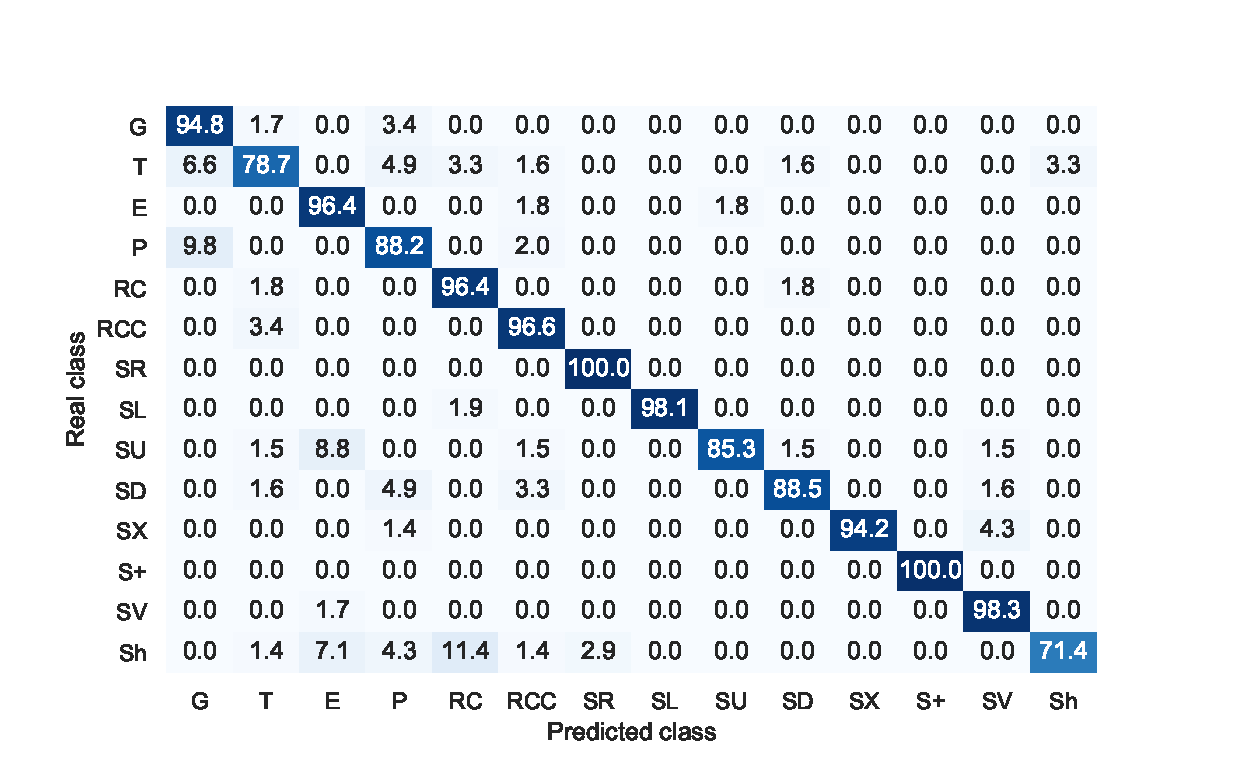
\includegraphics[width=\linewidth]{img/confusion-matrix-14-relative.eps}
        \caption{14 gesture classes case}
    \end{subfigure}
    \begin{subfigure}{\linewidth}
        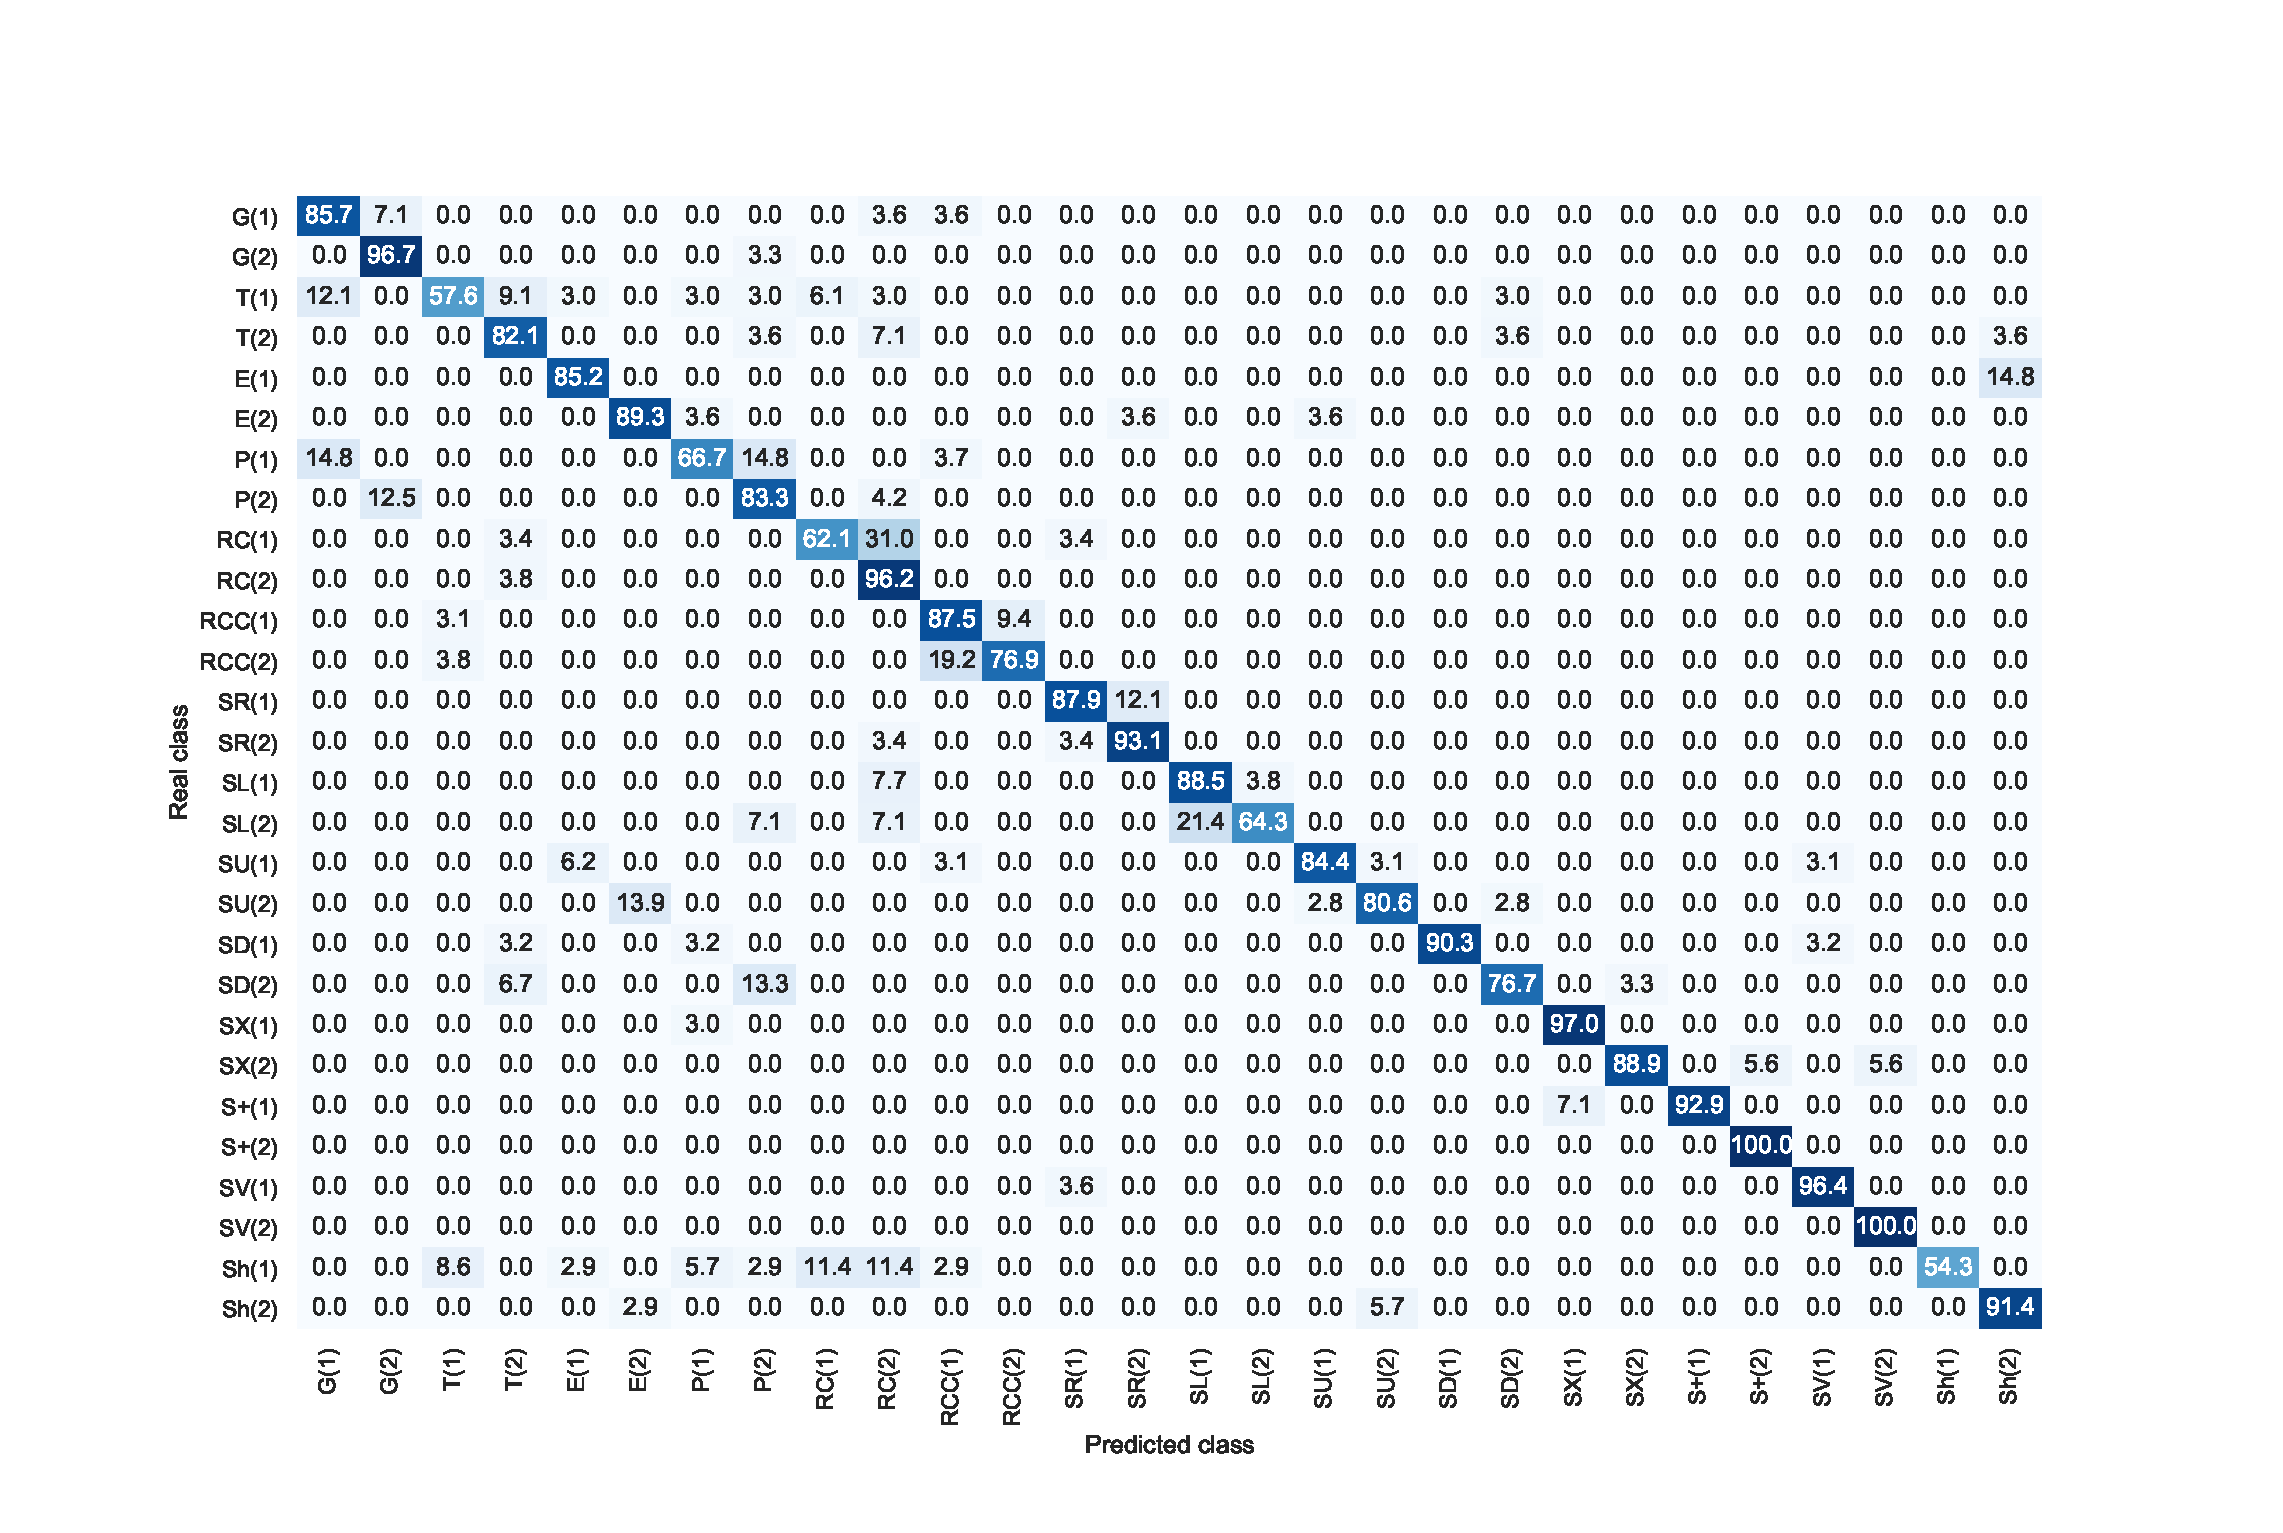
\includegraphics[width=\linewidth]{img/confusion-matrix-28-relative.eps}
        \caption{28 gesture classes case.}
    \end{subfigure}
    \caption{Confusion matrix of our regular CNN model on the DHG-14/28 test dataset. In the 14 gesture classes case we do not make a difference between using 1 finger and the whole hand, whereas we do in the other case.}
    \label{fig:confusion-matrix}
\end{figure}

\paragraph{TCN}
Even though we did not have time to fine tune the TCN architecture as well as the regular CNN one, the accuracy is very similar, and could probably surpass the regular CNN architecture. However, the model is considerably larger and slower to train.


\section{Discussion}
This work indicates that relatively small and shallow convolution network architectures can achieve good performance on skeletal data for gesture recognition.
It would interesting however to push the study further, notably by :
\begin{itemize}
    \item Adding a spatial and/or temporal attention mechanism, which seems to improve performance \cite{STA-Res-TCN} by giving more importance to the more interesting parts of the sequences. Our first experiments in that direction did not work well, however it could interesting to investigate further.
    \item Testing our model on other datasets, to see how well it generalizes.
    \item Using the model for real-time, step-by-step classification.
\end{itemize}




\bibliographystyle{plain}
\bibliography{sources}


\end{document}
